%!TEX root = ../Demo.tex
\chapter{预备知识}

在进行本文的叙述之前,需要预先了解一些相关的知识和定义,以便于使用更加简洁的描述方式。

德国数学家在 1874 年提出集合论(set theory),经过长时间的发展和完善,集合论成为了数学的一个重要组成部分,并且已经渗透到许多领域。计算机科学出现并发展壮大的过程中,集合论也成为计算机理论的一个重要基础概念。

集合论的最基础的概念是集合,集合的一个非形式描述为:一定范围内确定的,并且彼此可以区分的对象汇集在一起形成的整体叫做集合(set)\cite{book1}。



%%%%%%%%%%%%%%%%%%%%%%%%%%%%%%%%%%%%%%%%%%%%%%%%%%%%%%%%%%%%%%%%%%%%%%%%%%%%%%%%%%%%%%%%%%%%%%%%%%%%%%%%%%%%%%%%%%%%%%%%%%%%%%%%%%%%%%%%%%%%%%%%%%%%%%%%%%%%%%%%%%%%%%%%%%%%%%%%%%%%%%%%%%%%%%%%%%%%%%%%
\section{基本定义}

\begin{definition}[幂集\cite{watson1993taxonomyb}] \label{pro:mathP}
    对于任意集合$A$,我们使用$\mathcal{P}(A)$代表$A$的所有子集。$\mathcal{P}(A)$也叫做$A$的幂集。有时也写作 $2^A$。
\end{definition}

\begin{example}[集合的幂集]
    设集合 $A=\{a,b\}$,那么 $ \mathcal{P}(A) = \{\emptyset,\{a\},\{b\},\{a,b\} \} $,$\mathcal{P}(A)$ 等价于 $2^A$。
\end{example}

\begin{definition}[函数集\cite{watson1993taxonomyb}]
    对于集合 $A$ 和 $B$ ,$A\to B$代表所有从$A$到$B$的函数的集合。
\end{definition}

% \begin{definition}[等价类]
%     something to write。
% \end{definition}

\begin{definition}[等价关系的等价类\cite{watson1993taxonomyb}]
    对任何集合 $A$ 上的等价关系 $E$,我们使用 $[A]_E$代表等价类\footnote{等价关系和等价类稍后说明} 集合,即:
$$ [A]_E = \{ [a]_E :a \in A \} $$
集合 $[A]_E$ 也叫做 $A$ 的由 $E$ 引出的划分(partition)。
\end{definition}

\begin{definition}[等价类的指数\cite{watson1993taxonomyb}]
    对于集合$A$上的等价关系$E$,定义$\sharp E = | [A]_E |$。$\sharp E$ 也叫做$E$的“指数”。
\end{definition}


\begin{definition}[字母表\cite{watson1993taxonomyb}] \label{def:Alphabat}
    字母表是有限大小的非空集合。
\end{definition}

\begin{definition}[等价关系的细化]
    对于等价关系$E$和$E'$(在集合$A$上),当且仅当$E \subseteq E'$,$E$是$E'$的细化(refinement)。
\end{definition}













%%%%%%%%%%%%%%%%%%%%%%%%%%%%%%%%%%%%%%%%%%%%%%%%%%%%%%%%%%%%%%%%%%%%%%%%%%%%%%%%%%%%%%%%%%%%%%%%%%%%%%%%%%%%%%%%%%%%%%%%%%%%%%%%%%%%%%%%%%%%%%%%%%%%%%%%%%%%%%
\section{有限自动机}

本小节中定义有限自动机、其性质和用于有限自动机的变换。本节内容大部分直接引用自\cite{watson1993taxonomyb}。

\begin{remark}[状态转移图\cite{watson1993taxonomya}]
    一般来说,我们使用状态转移图来表示一个自动机,如图\ref{fig:state_graph}
\end{remark}

% 一般来说,我们使用状态转移图来表示一个自动机,如图\ref{fig:state_graph}

\begin{figure}[!htbp]
    \centering
    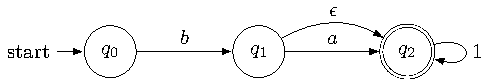
\includegraphics[width=0.7\textwidth]{state_graph}
    \caption{自动机状态转移图}
    \label{fig:state_graph}
\end{figure}

图\ref{fig:state_graph}中,自动机由$q_0$进入,接收字符“b”转移到状态$q_1$,状态$q_1$接收字符“a”转移到状态$q_2$,图中的两个同心圆圈住状态$q_2$表示结束状态( final state )或者接受状态( accepted state ),意味自动机处理字符串到达此状态时,自动机就接受当前处理的字符串,状态$q_2$上有一个指向自己的箭头,意为接收字符“1”之后,仍然指向自己。而状态$q_1$经过$\epsilon$转移到状态$q_2$,意为状态$q_1$可以不接收任何字符即可转移到状态$q_2$。图\ref{fig:state_graph}中的自动机接受的字符串为$\mathcal{L}=ba(1)^*\cup b(1)^*$。

\begin{definition}[有限自动机 \cite{watson1993taxonomyb}]
    有限自动机(Finite Automata,FA)是一个6元组$(Q,V,T,E,S,F)$,其中
    \begin{itemize}
        \item $Q$ 是有限状态集;
        \item $V$ 是一个字母表;
        \item $ T \in \mathcal{P}(P\times V \times Q) $是一个转移关系;
        \item $ E \in \mathcal{P}(Q\times Q)$ 是一个$\epsilon$-转移关系(空转移,不需要接收字符即可转移);
        \item $ S \subseteq Q $是开始状态集;
        \item $ F \subseteq Q $是结束状态集;
    \end{itemize}
    字母表和函数$\mathcal{P}$的定义分别在“定义\ref{def:Alphabat}” 和 “定义 \ref{pro:mathP}”。
\end{definition}

\begin{example}
    我们可以用$M=(\{q_0,q_1,q_2\},\{b,a,1,\epsilon\},T,E,\{q_0\},\{q_2\})$来指代图\ref{fig:state_graph}中的自动机。其中,$T=\{(q_0 \times b \times q_1),(q_1\times a \times q_2),(q_2\times 1 \times q_2)\}$,$E=(q_1 \times q_2)$。
\end{example}

\begin{remark}
    为了在某些情况下方便的展示状态之间的关系,也把状态转移图写成表格\cite{book1},如图\ref{fig:state_graph}中的自动机,写成表格\ref{tab:sample}:
\begin{table}[!htbp]
    \caption{状态转移函数}
    \label{tab:sample}
    \centering
    \small% fontsize
    \setlength{\tabcolsep}{4pt}% column separation
    \renewcommand{\arraystretch}{1.2}%row space 
    \begin{tabular}{l p{4em}<{\centering} p{1em}<{\centering} p{1em}<{\centering} p{1em}<{\centering} p{1em}<{\centering}} 
        \toprule%\hline 
        \multirow{2}{*}{状态说明} & \multirow{2}{*}{状态} & \multicolumn{4}{c}{输入字符} \\
		\cline{3-6}      &    &$a$ & $b$ & $1$ & $\epsilon$ \\
        %                        &        & \multicolumn{4}{c}{输入字符} \\
        %\cline{3-6}  {状态说明}  & {状态} &$a$ & $b$ & $1$ & $\epsilon$ \\
        \midrule%\hline
        开始状态(start)  & $q_0$ & -     & $q_1$  &      - &     -    \\
                        & $q_1$ & $q_2$ &    -   &    -   &    $q_2$ \\
        结束状态(final) & $q_2$ &   -   & -      & $q_2$  &    -     \\
        \bottomrule%\hline 
    \end{tabular}
\end{table}
\end{remark}


%\newpage
表格\ref{tab:sample}的状态之间的关系与$T=\{(q_0 \times b \times q_1),(q_1\times a \times q_2),(q_2\times 1 \times q_2)\}$,$E=(q_1 \times q_2)$一一对应,“\mbox{-}” 表示没有相应的转移关系。下文中将表格\ref{tab:sample}简称为转移函数。

\begin{remark}[转移关系的表示]
    为了更加简洁的描述转移关系,用 “$T=(q_0 \times b \times q_1)$” 来代表图 \ref{fig:state_graph} 中的 “状态 $q_0$ 接收字符 ‘b’ 转移到状态 $q_1$”。
\end{remark}

\begin{remark}
    本文在不同情况下使用不同的形式来表示转移关系,比如
\end{remark}

\subsection{有限自动机的性质}

本节定义有限自动机(Finite automata,下称 FA)的性质,为了使定义更加简洁,引进三个FA: $M=(Q,V,T,E,S,F)$ , $M_0=(Q_0,V_0,T_0,E_0,S_0,F_0)$ , $ M_1=(Q_1,V_1,T_1,E_1,S_1,F_1) $。

\begin{definition}[FA 的大小]
    定义一个FA的大小为$|M|=|Q|$。
\end{definition}

\begin{definition}[FA 的同构$\cong$]
    我们把同构定义为FA的等价关系。当且仅当 $V_0=V_1$,并且存在双射$g\in Q_0 \longrightarrow Q_1$ ,使得
\begin{itemize}
    \item $T_1 = \{ (g(p,q),a,g(q)) : (p,a,q) \in T_0 \}$
    \item $E_1 = \{ (g(p,q),a,g(q)) : (p,q) \in E_0\}$
    \item $S_1 = \{ g(s):s\in S_0 \}$
    \item $F_1 = \{ g(f):f\in F_0 \}$
\end{itemize}
时$M_0$和$M_1$是同构的(写作$M_0 \cong M_1$)。
\end{definition}

\begin{definition}[转移关系 $T$ 的扩展]
    我们把$T \in V \longrightarrow \mathcal{P} (Q \times Q) $ 到 $ T^* \in V^* \longrightarrow \mathcal{P} (Q \times Q)  $的转换关系以如下方式扩展: 
    \[ 
        T^*(\epsilon) = E^* 
    \]
    且对于$(a\in V,w\in V^*)$ 有 
    \[ 
        T^*(aw) = E^* \circ T(a) \circ T^*(w)    
    \]
    操作符$\circ$在惯例 A.5 中定义。
\end{definition}

\begin{definition}[左语言和右语言 \cite{watson1993taxonomyb}]
    状态($M$中)的左语言由函数$ \overleftarrow{\mathcal{L}} _M \in Q \longrightarrow \mathcal{P}(V^*)$ 给出,其中:
    \[ 
        \overleftarrow{\mathcal{L}}_M (q) = ( \cup s:s \in S : T^*(s,q) )  
    \] 
    状态($M$中)的右语言由函数$ \overrightarrow{\mathcal{L}} _M \in Q \longrightarrow \mathcal{P}(V^*)$给出,其中 
    \[ 
        \overrightarrow{\mathcal{L}}_M (q) = ( \cup f:f \in F : T^*(q,f) ) 
    \] 
    通常在没有歧义的时候移除下标$M$。
\end{definition}

\begin{definition}[ FA 的语言 \cite{watson1993taxonomyb}]
    有限自动机的语言由函数 $\mathcal{L}_{FA} \in FA \longrightarrow \mathcal{P}(V^*) $给出,该函数的定义为式 \ref{eq:languageoffa}: 
    \begin{equation}\label{eq:languageoffa}
        \mathcal{L}_{FA} (M) = (\cup s,f:s \in S \land f \in F : T^* (s,f))
    \end{equation}
\end{definition}

\begin{example}[FA 的语言]
    图 \ref{fig:state_graph} 中的 FA 接受的语言为 $ \mathcal{L}= \{ ba(1)^*\cup b(1)^* \}$。
\end{example}

\begin{definition}[完全 FA ($Complete$)]
    一个完全 FA 满足式 \ref{eq:complete} :
    \begin{equation} \label{eq:complete}
        Complete(M) \equiv ( \forall q,a:q\in Q \land a \in V : T(q,a) \not= \emptyset ) 
    \end{equation}
\end{definition}

\begin{definition}[$\epsilon$-$free$]
    当且仅当 $E=\emptyset$时,$M$ 是 $\epsilon$-$free$ 的。
\end{definition}

\begin{definition}[可达状态 \cite{watson1993taxonomya}]
    可达状态是 $M$ 中满足条件的状态的集合。分为 “开始可到达状态” 和 “可到达结束状态”,其中
    \begin{itemize}
        \item 开始可达状态:从开始状态可以到达的状态,写作 $SReachable(M)$;
        \item 可达结束状态: 能到达结束状态的状态,写作 $FReachable(M)$;
    \end{itemize}
    可达状态定义为:
    \[ Reachable(M) = SReachable(M) \cap FReachable(M) \]
\end{definition}

\begin{definition}[Start-useful 自动机\cite{watson1993taxonomyb}]
    一个 $Useful_s$ 自动机 定义如下: 
    \[ Useful_s (M) \equiv ( \forall q:q \in Q : \overleftarrow{\mathcal{L}} (q) \not= \emptyset ) \]
\end{definition}

\begin{definition}[Final-useful 自动机\cite{watson1993taxonomyb}]
    一个 $Useful_f$ 自动机 定义如下: 
    \[ Useful_f (M) \equiv ( \forall q:q \in Q : \overrightarrow{\mathcal{L}} (q) \not= \emptyset ) \]
\end{definition}

\begin{definition}[Useful 自动机\cite{watson1993taxonomyb}]
    $Useful$ 自动机是一个只有可达状态的 FA:
    \[ Useful (M) \equiv Useful_s (M) \land Useful_f (M) \]
\end{definition}

\begin{example}
    如图 \ref{fig:UsefulFA} 所示,其中
    \begin{itemize}
        \item 图 \ref{fig:UsefulFA-2} 为一个 $Useful$ FA;
        \item 图 \ref{fig:UsefulFA-1} 中状态 $q_1$ 不是一个开始可达状态,也称开始不可达状态(start-unreachable);
        \item 图 \ref{fig:UsefulFA-1} 中状态 $q_2$ 不是一个可达结束状态,也称陷阱状态(final-unreachable)\cite{watson1993taxonomyb}。
    \end{itemize}
\end{example}

\begin{figure}[!htbp]
    \centering
    \begin{subfigure}[b]{0.45\textwidth}
        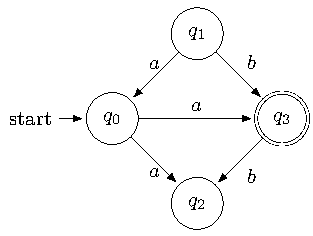
\includegraphics[width=\textwidth]{UsefulFA-1}
        \caption{}
        \label{fig:UsefulFA-1}
    \end{subfigure}
    ~
    \begin{subfigure}[b]{0.45\textwidth}
        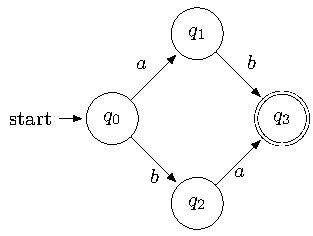
\includegraphics[width=\textwidth]{UsefulFA-2}
        \caption{}
        \label{fig:UsefulFA-2}
    \end{subfigure}
    \caption{}
    \label{fig:UsefulFA}
\end{figure}

\begin{definition}[确定性有限自动机 \cite{watson1993taxonomyb}]
    当且仅当 
    \begin{itemize}
        \item 无多重开始状态;
        \item 无$\epsilon$转移;
        \item 转移函数$T \in Q \times V \longrightarrow \mathcal{P} (Q) $ 不将 $Q \times V$ 映射至多重状态。
    \end{itemize}
    时有限自动机$M$是确定性的,称 $M$ 为确定性有限自动机(Deterministic Finite Automata,下称 DFA)。
    公式形式表达为式 \ref{eq:DetFA} :
    \begin{equation}\label{eq:DetFA}
    Det(M) \equiv ( |S| \leq 1 \land \epsilon\mbox{-} free(E) \land ( \forall q,a:q \in Q \land a \in V : |T(q,a)| \leq 1 )) 
    \end{equation}
    且有$ DFA \subseteq FA$。
\end{definition}


\begin{definition}[DFA 的最小化]
    满足以下条件时,$M\in DFA$是最小的:
    { \small \[  Min(M) \equiv (\forall M' : M' \in DFA \land Complete(M') \land \mathcal{L}(M) = \mathcal{L}_{FA}(M') : |M| \leq |M'| ) \] }
函数 $Min$ 仅定义在 DFA 上。一个最小的但是仍然完全的 DFA 的定义如下:
{\small \[  Min_{\mathcal{C}}(M) \equiv ( \forall M':M' \in DFA \land Complete(M') \land \mathcal{L}_{FA}(M) = \mathcal{L}_{FA}(M'): |M| \leq |M'| ) \] }
$Min_{\mathcal{C}}$ 仅定义在完全 DFA 上。
\end{definition}

\subsection{有限自动机的变换}

\begin{transformation}[FA 的反转(reversal)]
        $FA$反转由上标函数$ R \in FA \to FA $ 给出,它的定义如下:
        \[ (Q,V,T,S,F)^R = (Q,V,T^R,E^R,F,S) \]
    函数 $R$ 满足
    \[ (\forall M : M \in FA : ( \mathcal{L} (M) )^R = \mathcal{L}_{FA}(M^R)) \]
\end{transformation}

\begin{transformation}[移除开始状态不可达状态]
    变换$useful_s \in FA \longrightarrow FA$移除开始状态不可达状态:
    \begin{table}[!htbp]
        \centering
        \small% fontsize
        \setlength{\tabcolsep}{4pt}% column separation
        \renewcommand{\arraystretch}{1.4}%row space 
        \begin{tabular}{lcll} 
            $useful_s(Q,V,T,E,S,F)$ & = & {\bfseries let} & $U = SReachable(Q,V,T,E,S,F)$ \\
                                    &   & {\bfseries in}  &                               \\
                                    &   &                 & $(U,V,T \cap (U\times V \times U), E \cap (U \times U), S \cap U, F \cap U )$  \\
                                    &   & {\bfseries end} &                               \\
        \end{tabular}
    \end{table}
\\函数 $ useful_s $满足
\[  (\forall M : M \in FA : Useful_s ( useful_s(M) ) \land \mathcal{L}_{FA} (useful_s(M)) = \mathcal{L}_{FA}(M)) \]
\end{transformation}

\begin{transformation}[子集构造]
    函数$subset$把一个$\epsilon$-$free$ $FA$ 转换为一个 $DFA$ (in the \textbf{let} clause $T'\in \mathcal{P}(Q) \times V \longrightarrow \mathcal{P}(\mathcal{P} (Q) )$): 
    \begin{table}[!htbp]
        \centering
        %\small% fontsize
        \setlength{\tabcolsep}{4pt}% column separation
        \renewcommand{\arraystretch}{1.4}%row space 
        \begin{tabular}{lcll} 
            $subset(Q,V,T,\emptyset,S,F)$ & = & {\bfseries let} & $T'(U,a) = \{ (q:q\in U : T(q,a) ) \} $ \\
                                          &   &                 & $F'= \{ U : U \in \mathcal{P}(Q) \land U \cap F \not= \emptyset \} $ \\
                                          &   & {\bfseries in}  &                                         \\
                                          &   &                 & $ ( \mathcal{P}(Q),V,T',\emptyset,\{ S \},F' ) $  \\
                                          &   & {\bfseries end} &                               \\
        \end{tabular}
    \end{table}
    \\有时候也把它说成“幂集”构造。
\end{transformation}



\section{等价性和最小化}